\subsubsection{Belarus}

\paragraph{Outline}
\begin{enumerate}
    \item Cyclic -> can strategize in picks and for kill-rates 
    \item Map is brawly. Safe remote +3s in corners. E/S too safe, less expansion and flexibility. W/N more flexible, more expansion, less safe. Central +3s relative to distribution.
    \item +4s great at a) FTBs if you can survive Turns 2-4, b) at safe pivot picks for income regions in bad distributions, c) good for 12 in two, d) for positional play and counter with precision (e.g. opponent picks red +3 FTB north with +4 below it, expands into +4 T3, plans to complete T4, you surprise them with a counter out of thin air from Narnia).
    \item Can find perfect picks.
    \item Position and army advantage are everything.
    \item Beware WR bullshit eliminations on 12vs12, 7vs7 etc fronts.
\end{enumerate}
\paragraph{Map Dynamics}

\begin{figure}[H]
  \centering
  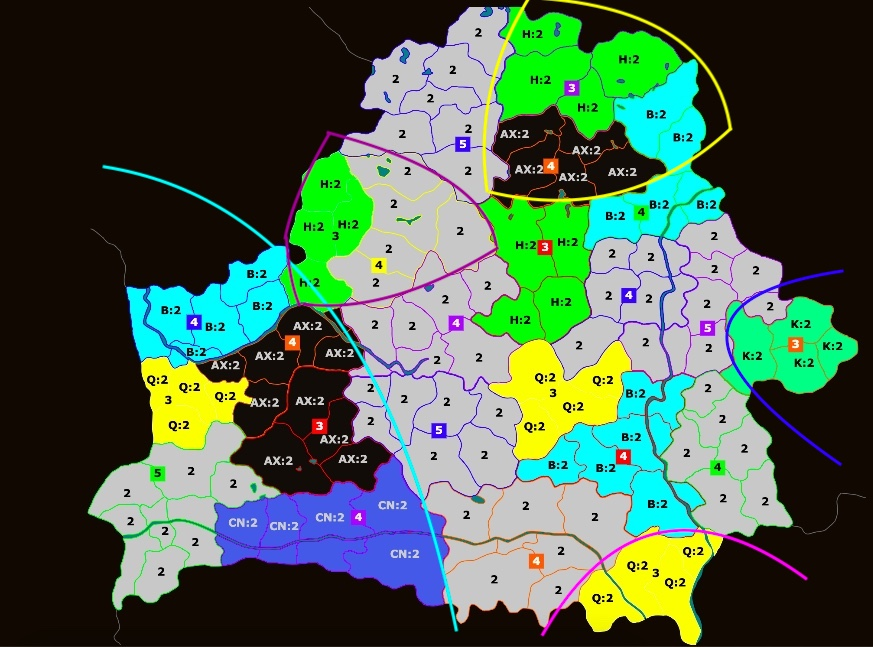
\includegraphics[width=0.8\textwidth]{Images/Belarus.jpg}
  \caption{Bonus Win Rates and Regions for Games with Overall Winner Rating >=1800 in Belarus(n=428) (AX> all. CN>B>- for +4 bonuses. H>K>Q>- for +3 bonuses.)}
  \label{belarus_regions}
\end{figure}

Belarus is a WR Brawl template and anyone saying differently is lying. Safety is an illusion, best represented maybe with a game like \href{https://www.warzone.com/MultiPlayer?GameID=36572705}{this} where you build the stack and go in.
\\
\\
Having said that, there is relative safety, which has a lot to do with the settings of the map. You've got 6 initial armies, enough for expansion immediately, and 5 base Income. In this premise, you can even get 2x +3 bonuses by end of T2, making the +3 bonuses very desirable. On top, because the map is a brawl and within 2-3 steps you can reach anything, the edges are more attractive (in most cases again efficient +3 bonuses). As a result there are sort of 2 generic categories of distributions. First, the exception, is distributions that offer dominating +3 or +4 FTBs or combos.For example \href{https://www.warzone.com/MultiPlayer?GameID=35888891}{in AWP 2023 Finals, Top2, Game 1}, Phaeril just triple picks a +4 in the center and wins in 5 turns. Second, is a mixture of distributions where you want to get a balance between positional advantage and income advantage upon contact. Sometimes that involves picking the FTBs/combos and fighting on T1, T2 etc. Examples \href{https://www.warzone.com/MultiPlayer?GameID=40269350}{here} and \href{https://www.warzone.com/MultiPlayer?GameID=36572705}{here}. Sometimes you can sneak safe picks in remote regions and just cover the FTB, as for example \href{https://www.warzone.com/MultiPlayer?GameID=40398807}{here}, 1/2 a safe region 3/4/5/6 in a contested area.  

The colors on Figure \ref{belarus_regions} depict the WR of each bonus differentiating between +4 and +3 bonuses. Looking at them separately:
\begin{itemize}
    \item The +3 bonuses are flexible. There's a total of 8.
    \begin{enumerate}
        \item 2 West
        \item 1 Far North
        \item 1 Far East
        \item 1 Far South
        \item 3 closer to the center
    \end{enumerate}
    \item Evaluating which is best has to do with what's your goal.
    \begin{enumerate}
        \item The Far South +3 is very safe (for example \href{https://www.warzone.com/MultiPlayer?GameID=36672825}{here} Hergul tries to get 2 remote +3 bonuses and contest the West with 3/4/5/6 and it works), but cannot be used to flank income (2 steps for a single border to 1 useful bonus in the center) and it's expansion is sort of slow and not safe. You'd want to pivot to income away from your opponent not towards them, like \href{https://www.warzone.com/MultiPlayer?GameID=36792398}{here}.
        \item The Far East +3 serves the exact same purpose as above, but has better expansion and reachability. For example \href{https://www.warzone.com/MultiPlayer?GameID=32481090}{here} there's 1 FTB in the board and a lot of contested income (either on T1 or T2), so you cannot deviate. Another example \href{https://www.warzone.com/MultiPlayer?GameID=32247185}{here} where the distribution is as boring as one can get with 2 FTBs left and right.
        \item The North +3 and two West ones are superior for controlling income zones and expanding.
        \item The central ones are situational, typically for FTBs, combos or counters
    \end{enumerate}
    \item The +4 Bonuses act similarly but combo differently. We established already that a) +3s enable more income earlier due to how they combo with 6 starting armies for 11 end of T2 and b) they conveniently are placed and scattered in the safest corners of the map. +4s require different setup. In +3 FTB distributions +4s are complementary and counter-focused, but in more open distributions they are great for expansion beyond the first turn. As for example \href{https://www.warzone.com/MultiPlayer?GameID=30166708}{here} where Octane set ups 12 in two and a solo pick +4 that has great linear expansion away from the opponent towards goood bonuses. 
\end{itemize}



\paragraph{Picking Logic}

Belarus has a weird distribution system I'll explain in this paragraph. Map of 118 territories and 23 bonuses with neutrals of 3 and RWD. Random RWD means the engine finds a territory in each bonus to distribute, so 23 initial territories. On top, the neutrals in distribution - territories no-one picked, become 2 army neutrals, as well as there are 35 wastelands of 2. If the territory that was supposed to be distributed is a wasteland of 2, then that bonus has no spawwn. For example \href{https://www.warzone.com/MultiPlayer?GameID=40269350}{here} you can clearly see that at the south, amongst other areas, red +4 and yellow +3 don't have a spawn but have 2 and 1 wasteland of 2 respectively. As a result, Belarus distributions differ a lot from game to game.
\\
\\
Given that Belarus is WR, thinking about kill-rates is torture, but 3 army neutrals and Cyclic move order help a lot in identifying whether or not you can force a line or not. For example \href{https://www.warzone.com/MultiPlayer?GameID=34663752}{here} the game is a question of whether or not you can afford not picking the +4 FTB in the west. Get your notebook out.
\begin{itemize}
    \item From Bechaa's POV, approaching the first 2 turns similarly to his gameplay, we are set to arrive on the double border end of T2 with 9, 8 or 7. 81\% to arrive with 9, 18\% to arrive with 8, 1\% to arrive with 7. (91\% from 0.9 x 0.9) and without knowing move order.
    \item From Octane's POV, same gameplay, 2 attacks that matter for us and assuming we get the 90\% roll on the T1 attack to Skidziel for the leftovers that will be used on the +3 on T2. Two attacks take place, the 5v2 and 4v2 from where the leftovers go towards the double border. Each attack comes with 60\% chance to get -1 attacker, 40\% chance for -2 attackers. Octane stacks the leftovers in Skidziel Turn 2 because you expect the counter. From those two attacks, 36\% chance to have in Skidziel 6, 48\% chance to have 5 and 16\% chance to have 4 (what happened in the game. The position heavily favors Octane it is close to a forced win.
    \item If bechaa doesn't flip the game on a first move break on T3, he literally can never break, it is surrender-able on Turn 4, and that's with Octane getting the 16\% chance scenario. If Octane get's the 36\% roll, Bechaa cannot even flip the game with the T3 kamikaze all in. And all this is only possible 81\% of the times Bechaa arrives with 9 in the double border. 
    \item So, it's a matter of whether this is a solid strategy or not, that is picking acknowledging that your entire position relies on a T3 flip that can work only if my opponent gets bad rolls <50\% of the time). If you are a 1600 player and do this against Rufus honestly good for you if you recognize that getting lucky is your best path to a victory. But in the path to improve you have to get serious.
\end{itemize}

The argument at the end of the day and point I would make is that in the hands of a calculative player, a combo or a triple pick is more powerful and you can extent the logic of forcing plays in certain turns to optimizing picks thinking of turns in advance.  From T4 onwards Octane has won and the easiest way to convert is to block Bechaa's potential all in T4 of 13 armies (defend with 9) and attacking from both territories in the same cycle - no attack in between. When you calculate the position you'll find that despite no RF on T5, by the time bechaa breaks the bonus, he will be at some an army disadvantage that the game will be easier to convert.
\\
\\
\textbf{2x +2 FTBs}
A typical distribution of 2 FTBs will look like \href{https://www.warzone.com/MultiPlayer?GameID=32247185}{this} and the eternal question is how to pick these configurations. Both approaches you see in the game are sound and it really is a matter of gameplay and luck. I personally prefer Crazy's approach but with a different idea behind it. The 1/2 combo 3 safe 4/5/6 coverage approach counters the 1/2 combo 3/4/5/6 coverage and 1/2 combo 3/4 combo 5/6 combo approach due to ending up in a position where you have 2 contested spawns and your opponent has 3 contested spawns, with the downside that you have an army disadvantage early. Ideally, when you get a 1turn away counter to an ftb, you want something closer to \href{https://www.warzone.com/MultiPlayer?GameID=36672825}{this}, because you prepare your attack, and align it with a stack and your opponent committing elsewhere. Specifically in the distribution above between Crazy and Timi, Crazy cannot afford such an option, as Timi can complete the +3 FTB west with 0 deployments. Had the neutrals been 3, different kill-rates, different strategies. Same idea \href{https://www.warzone.com/MultiPlayer?GameID=26364060}{here}, Beep gets his 6th and uses it to counter a region from T4 onwards, when he knows the counter will succeed
\\
\\
+3 FTBs dictate how to pick but aren't mandatory. \href{https://www.warzone.com/MultiPlayer?GameID=25238378}{here} Octane goes for 1/3 safe +3 ftb, 2/4 not so safe +3 ftb, 5/6 ftb that's in the center. Rufus' picks opt precisely to get 1/2/4 or 2/3/4 and get to 11 income end of T2 to block Octane's expansion. More income on the turn of contact is usually a good thing. Same exact concept \href{https://www.warzone.com/MultiPlayer?GameID=30348571}{here}. There are 4 ftbs on the board across the 4 directions. Mori 2/3 picks the safest, and first picks the +3 that can be used to counter the expansion of the west FTB. He gets 1/2/3 and get's an 11v8 contact end of turn 2 (but Ryiro outsmarts him picking the counter to Mori's ftb expansion and north +3 ftb. Though still not countering on T4 but T5 is risky but works). Pretty much the same concept again but with different bonuses from \href{https://www.warzone.com/MultiPlayer?GameID=30699151}{Buns}.
\\
\\
\textbf{+4 FTBs}
+4 are really strong and you should either cover them, pick them, or pick to counter them. Picking them is as straight forward as Phaeril's AWP finals game in the above section. Covering them is tricky and that's where Figure \ref{belarus_regions} can help. Some +4 bonuses are just better than others the ones in the west usually have immediate expansion and with 12 income end of T2 you are practically unstoppable (like Octane vs Bechaa example \href{https://www.warzone.com/MultiPlayer?GameID=34663752}{here}). In fact I take back "practically", you are mathematically unstoppable. Your opponent must have a counter further away in order to build a stack to hit harder or with better timing. As an example, \href{https://www.warzone.com/MultiPlayer?GameID=26364060}{Beep} in this game recognises that the +4 FTB goes up to 16 end of T4. He sets up going also to 16 end of T4 and countering that turn. Earlier won't work, later Timi is already on his way everywhere and might pivot. Another example \href{https://www.warzone.com/MultiPlayer?GameID=25698044}{here} Beep uses his 1st pick to stack and counter much later. 


\paragraph{Gameplay}

Same to every other WR template, find your win condition and play for it. The map is a brawl. As such you often can not pivot to different areas and have to fight multiple fronts. Belarus has cyclic move order, so you apply that to picks and strategies.
\\
\\
In \href{https://www.warzone.com/MultiPlayer?GameID=37430202}{AWP Finals QF} between Crazy and tornado, the board is lackluster, seen in Figure \ref{belarus_awp}.

\begin{figure}[H]
  \centering
  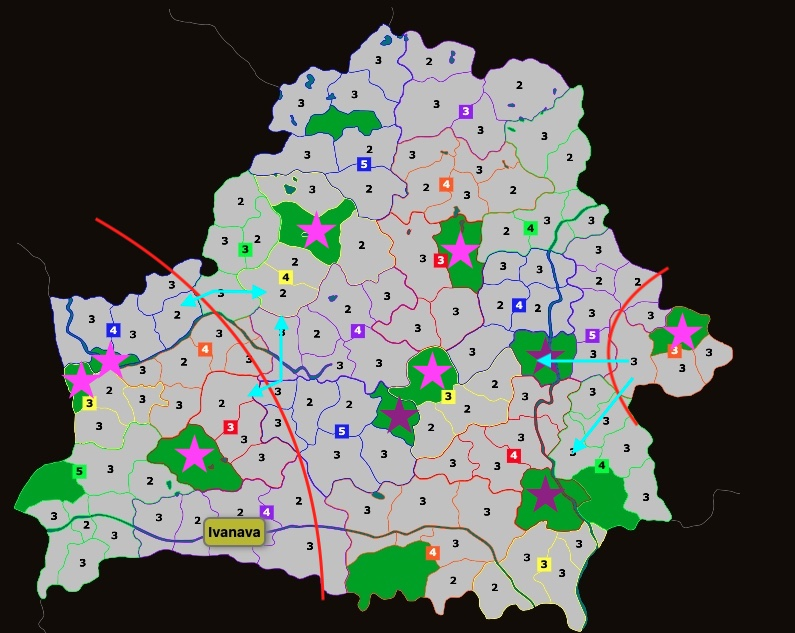
\includegraphics[width=0.8\textwidth]{Images/belarus_awp.jpg}
  \caption{Belarus Distribution,example 1}
  \label{belarus_awp}
\end{figure}

\begin{itemize}
    \item Picks: Simplify the board. North has nothing, south doesn't matter besides the red +4 that is directly countered by a contested yellow +3 ftb. We are down to West, Center and East.
    \item The West has 3 viable picks. Light Green +5 is troll, you counter a single border of the red +3 or hunt ghosts north where the opponent would rather get the blue +4 to begin with. 
    \begin{enumerate}
        \item Red +3 > Blue +4 if it gets the double border "Dzyatlava".
        \item Red +3 $\approx$ Yellow +3 single pick they break each other.
        \item Red +3 single pick > 2 picks for obvious reasons, your 2nd pick is somewhere else safe.
        \item Blue +4 enables 12 in 2 combos with Orange +3 east or blue +3 in the center. Blue +4 combo and red +3 center lose to yellow +3 center FTB or even yellow +3 center + red +3 west + yellow +4 due to the simple fact you get contact end of t2 12vs11 with a double border situation in your red +3. Blue +4 combo and orange +3 east get to 12 end of t2 without contact so it's sort of pointless, you'll move towards red +3 t3 hoping for contact but will probably be 12vs14/15 then in a position you can't convert. Opponent can even let their red +3 drop and flank in 1 turn blue +4 from north double border in "Iŭje"
        \item tldr: Blue +4 is spicy and no real good pairs. Red +3 better positionally
    \end{enumerate}
    \item East +3 is a safe bonus to fight elsewhere but has 0 flexibility, nor expansion. 
    \item In the center, the south red +4 is entirely dependent on the yellow +3 above it which is an FTB. To pick the red +4 there, I would personally start from a trap set like:
    \begin{enumerate}
        \item 1/2 blue +4 west, 3/4 yellow +3, and blue +5 center, 5 red +4 south and 6 purple +5. Or
        \item 1 red +3 west, 2 blue +4 west, 3/4 yellow +3 and blue +5 center, 5 red +4 south, 6 purple +5.
    \end{enumerate}
The idea is to setup a situation where I get 1/4/5 with a counter to the center that I can bait to get eliminated and use my 5 afterwards to imitate the meme "call an ambulance but not for me". Outside of such trap sets, the red +4 south is very reliant on the yellow +3 above it, which also conveniently pairs with the red +3 above (also a double border) for an FTB and is an FTB itself.
    \item As such, yellow +3 is a great first, it's position simplifies the game for you. 
    \item Building picks from there, it gets a bit ugly. You want to do 1 center 2/3 west 4/5/6 coverage instinctively but can lose the west, no real coverage for 4/5/6, need to think smarter. You can 100\% go for 1/2 west 3 orange +3 east 4/5/6 yellow +3 FTB coverage of center but run into a) 1/2/3 = defeat and b)Getting any iteration with 5 such as 1/3/5 , 1/2/5, gives 0 info on move order and you just lost a red +3 FTB in the center. On top, c) 1/4/5 you move 2nd turn 1, so having your counter to a 4th pick yellow +3 FTB is counter-intuitive given on top that c) you move 2nd and d) opponent out-delays turn 1 (abbaabba) with 3rd "a" a conditional tap. So let's just start with a given first pick to simplify things. Take into consideration that a) you can lose first pick and b) 2/3 isn't guaranteed coverage as you can get 1/4/5.
    \item Identify a series of sets with ideas in mind. Let's go for: (W:West, E:East, etc.)
    \begin{enumerate}
        \item a) Yellow +3 / E. Orange +3 / N. Yellow +4 / 456 West.
        \item b) Yellow +3 / Purple +5 / Blue +5 / 456 West
        \item c) Yellow +3 / W. Red +3 / W. Yellow +3 / N. Yellow +4 / Purple +5 / Blue +5
        \item d) Crazy's set
        \item e) tornado's set
    \end{enumerate}
    \item Play the sets out in your head and find out their weaknesses and strengths. For example
    \begin{enumerate}
        \item a). 1/2/3 is a positional loss in the long run with 3 spawns in the center/east and 0 coverage west. If no contact in blue +5 you risk 11 in two, complete yellow +4 t3 hopefully and try to counter the west from yellow +4. Issue is purple +5 that directly counters 2 of your picks. Losing fp is sad, as you might've just lost 1 or 2 FTBs in the center. 2/3/6 works. a) vs b) doesn't matter b) is a troll set, a) vs c),d),e) you over-commit on the east with two picks that get countered by the purple +5
        \item c) vs e) you get either 
        \begin{itemize}
            \item c: yellow +3/purple +5 FTB, W: yellow +3 vs e: W: red +3, N: yellow +4, N: red+3
            \item e: yellow+3/red+3 FTB, yellow +4 vs c: W: red +3/yellow +3, purple +5.
        \end{itemize}
        \item c) gets first pick: c has FTB into yellow +3 west, 11 end of t2, but is far away from threatening income e) stabilizes at 12, tries to keep the game 12vs11 and c) has to foresee the flank north in 2 steps to triple border.
        \item e) gets first pick: e has FTB red +3 into yellow +4 that t3 immediately moves south, it's a race of who breaks who first. c) has purple +5 which is 3 steps away from single border into yellow +4 (assuming breaks). e) sees red +3 in 1 turn and had an FTB -> e has an advantage.
    \end{enumerate}
    \item Notice patterns in the gameplay that will rise up. And justify your picks accordingly. Tornado's 3/4 sets up a safe +4 north will accessibility west, but losing first pick always makes things ugly.
\end{itemize}

In the game:
\begin{itemize}
    \item Scatter your moves, it's WR. T1 red +3 west scatter of attacks is because a) if the 3 attack fails you can recapture with 2 and b) you can use either a tap or a mixture of 2\&2 to capture last territory, as Tornado's goal is 11 in two.
    \item All around tips. T3 tornado save even the 1 movable east. Crazy capture double border.
    \item T4 Crazy has to make a bold prediction. tornado knows it's 12vs9 in income and that he has first order. Crazy can first move with up to 17 -> tornado defense of 12 and survive east with rest. Crazy has to read the play and either a) full deploy west stay or b) predict tornado will use at least 9/12 deploys west->3 deploys east, gamble elimination.
    \item T5 the game now for tornado is about converting the 12vs9 into a win, the bonus on the west without a first order isn't as important, especially given the yellow +4 counter nearby. Shortest path to victory is deny your opponent any other bonus -> retain the 12vs9 lead till it's no longer playable. If he uses rf, all ins west +4 breaks it in 2 places but gets eliminated in the yellow +3 his armies are now in an awkward corner of the map where Crazy can just blockade and survive in yellow +3.
In short, find the path to victory.
\end{itemize}